\documentclass[11pt,letterpaper]{article}

\usepackage[margin=1in]{geometry}
\usepackage{amsmath,amssymb,mathtools}
\usepackage{booktabs,tabularx,array}
\usepackage{enumitem}
\usepackage{microtype}
\usepackage{tikz}
\usetikzlibrary{arrows.meta,positioning,calc}
\usepackage{listings}
\usepackage{hyperref}

\hypersetup{hidelinks}
\setlength{\parindent}{1.5em}
\setlength{\parskip}{0pt}
\setlist[itemize]{leftmargin=2em}
\setlist[enumerate]{leftmargin=2.2em}

\newcommand{\Rcal}{\mathcal{R}}
\newcommand{\Ccal}{\mathcal{C}}
\newcommand{\ind}{\mathbb{I}}
\newcommand{\softmax}{\operatorname{softmax}}
\newcommand{\ReLU}{\operatorname{ReLU}}

\lstdefinestyle{pseudocode}{
  basicstyle=\small\ttfamily,
  columns=fullflexible,
  keepspaces=true,
  frame=none,
  xleftmargin=1.5em,
  breaklines=true,
  captionpos=t
}

\title{\textbf{Adaptive Route Prediction on Dynamic Graphs:}\\
\textbf{A Two-Tier Candidate-Generation and Neural-Selection Framework}\\[0.7em]
\large A Framework and Design Paper}
\author{Krish Parikh (Lapenzer)\\
Independent Researcher, Ontario, Canada\\
\texttt{lapenzerparikh@gmail.com}}
\date{August 17, 2026}

\begin{document}

\maketitle

\begin{center}
Copyright \copyright\ 2026 Krish Parikh. All rights reserved.
\end{center}

\begin{abstract}
This paper develops a theoretical framework for predicting an entity's next movement or complete route on a dynamic directed graph. The first tier constructs a constrained and diverse candidate set from generalized-cost search, loopless $K$-path deviations, transition priors, node frequency, stochastic routing, destination progress, and contextual resistance. The second tier assigns a learned selection score to each candidate and converts the scores into a probability distribution over the candidate set. Population and entity-specific histories are combined through a shrinkage rule, while time-varying context enters a sign-constrained utility model. The formulation includes definitions of confidence, entropy, calibration, selective prediction, and abstention.

For every finite candidate distribution, the expected route length is proved to lie between the shortest and longest candidate lengths; when edge length is metric, the direct source--target distance provides an additional lower bound. A terrain and contour-graph module extends generalized resistance without treating contour lines themselves as routes. The paper also defines a prospective evaluation methodology that separates candidate recall, next-node accuracy, full-route accuracy, probabilistic calibration, selective risk, and operational availability. No implementation, dataset, fitted model, or empirical result is presented. Accordingly, the contribution is a framework and research design whose claims are mathematical and methodological.
\end{abstract}

\noindent\textbf{Keywords:} route prediction; dynamic graphs; $K$-shortest paths; transition models; node frequency; neural ranking; selective prediction; uncertainty

\section{Introduction}

Route prediction extends beyond geometric shortest-path computation. A traveller, vehicle, response team, packet, or other moving entity may prefer familiar nodes, avoid adverse conditions, preserve access to intermediate resources, or react to constraints that change during movement. A useful model therefore represents network structure, historical behaviour, and time-varying context within a common decision process.

The Route Prediction Algorithm (RPA) formalizes that process on a dynamic directed graph. Multiple independent models propose or assess plausible movements. A second tier learns how their signals interact with context. Separating candidate generation from selection keeps structural constraints inspectable while permitting a context-sensitive ranking rule. The model also allows an abstention outcome when the candidate set, data state, or score distribution does not support a sufficiently confident decision.

The theoretical contributions are:

\begin{enumerate}
  \item a dynamic-graph formulation with explicit feasibility, loop, and immediate-backtracking constraints;
  \item a generalized resistance function that combines geometry, history, context, access, risk, exposure, terrain, and resource variables under explicit sign conventions;
  \item a two-tier architecture that separates diverse candidate generation from learned candidate selection;
  \item population and entity-specific transition priors joined by data-dependent shrinkage, together with a distinct node-frequency prior and destination-progress term;
  \item a formal route-length bound, a normalized candidate distribution, and definitions of confidence, entropy, and abstention; and
  \item a proposed evaluation design that distinguishes candidate coverage, next-node performance, complete-route performance, calibration, selective risk, and availability.
\end{enumerate}

This manuscript deliberately stops at theory and design. Section~\ref{sec:standing-requirements} specifies the standing requirements that a separate results-bearing companion paper would have to satisfy.

\section{Related Work}

Shortest-path search and loopless $K$-path enumeration provide the structural foundations for candidate generation \cite{dijkstra1959,yen1971}. Recent route-choice research adds complementary ideas. Yao and Bekhor combine data-driven choice-set generation with discrete-choice estimation \cite{yao2020}; their work is closest to the proposed separation between candidate construction and selection. Zhao and Liang use inverse reinforcement learning to recover context-dependent link rewards \cite{zhao2023}, whereas the present framework makes its resistance and utility terms explicit. RoutesFormer represents complete link sequences with a Transformer \cite{qiu2024}; this is an alternative sequence-based selector once a route representation is fixed. Wang, Moylan, and Levinson study path-based ensembles \cite{wang2024}, which motivates the transparent fixed ensemble used here as an interpretable comparator to a learned selector.

Motion-forecasting research addresses a neighbouring output space. LaneGCN encodes map topology as a lane graph \cite{liang2020}, Trajectron++ incorporates heterogeneous dynamics and feasibility \cite{salzmann2020}, and Scene Transformer models interactions among multiple agents \cite{ngiam2022}. Motion Transformer introduces intention queries for multimodal futures \cite{shi2022}, while Wayformer studies attention-based architectures across input modalities \cite{nayakanti2023}. These systems suggest richer selector families, but their continuous trajectories and displacement metrics differ from discrete graph-route prediction. Standardized resources such as the Waymo Open Motion Dataset and Argoverse~2 illustrate how future empirical work can fix scenes, maps, splits, and metrics \cite{ettinger2021,wilson2021}.

\subsection{Positioning Across Prediction Tasks}

Three related tasks should remain distinct: route-choice models estimate a path or next link from a network and context; motion-forecasting systems predict continuous future trajectories and associated probabilities; and graph-route ranking selects from an explicit, constrained candidate set. Table~\ref{tab:positioning} summarizes the relationship.

\begin{table}[htbp]
\centering
\caption{Methodological positioning of the framework.}
\label{tab:positioning}
\footnotesize
\begin{tabularx}{\textwidth}{>{\raggedright\arraybackslash}p{0.22\textwidth} >{\raggedright\arraybackslash}p{0.21\textwidth} >{\raggedright\arraybackslash}p{0.22\textwidth} X}
\toprule
\textbf{Work family} & \textbf{Prediction unit} & \textbf{Typical evaluation} & \textbf{Relation to this framework} \\
\midrule
Choice-set and discrete-choice models \cite{yao2020,wang2024} & Whole path from an enumerated set & Choice likelihood, hit rate, held-out choice accuracy & Closest analogue to Tier~1 and the fixed ensemble. \\
Link and sequence-route models \cite{zhao2023,qiu2024} & Next link or complete link sequence & Link accuracy, path accuracy, sequence likelihood & Direct comparison family for next-node and exact-route evaluation. \\
Graph-based multimodal motion models \cite{liang2020,salzmann2020,shi2022,nayakanti2023,ngiam2022} & Continuous multimodal trajectories & Displacement error, miss rate, probabilistic ranking metrics & Architecturally relevant, although the output space differs. \\
Standardized motion benchmarks \cite{ettinger2021,wilson2021} & Agent scenes, maps, and future trajectories & Fixed validation and test protocols & Templates for a future external evaluation, after aligning the task definition. \\
\bottomrule
\end{tabularx}
\end{table}

Cross-paper comparison requires a shared prediction unit, candidate space, split, and denominator. A route-choice comparison would apply every selector to identical graph candidates and decision events. A motion-forecasting comparison would first convert graph candidates to time-indexed trajectories and then apply the benchmark's official metrics. Classification accuracy alone also does not establish probability calibration; Brier score, negative log-likelihood, expected calibration error, and risk--coverage analysis remain necessary \cite{guo2017}.

\subsection{Requirements for a Comparable Future Experiment}

A comparable study fixes one decision-event key and a chronological, entity-grouped split. Every selector receives the same candidate set. Shortest path, most-frequent transition, population Markov, entity Markov, the fixed ensemble, and the neural selector are then scored on identical events. Common denominators make candidate recall, top-1 and top-$K$ next-node accuracy, exact-route accuracy, overlap, negative log-likelihood, Brier score, calibration, coverage, and latency interpretable across methods. Section~\ref{sec:standing-requirements} states the complete validation bar.

\section{Problem Definition}

\subsection{Dynamic Directed Graph}

At time $t$, represent the environment as a directed graph
\begin{equation}
G_t=(V_t,E_t,W_t),
\end{equation}
where $V_t$ is the set of available nodes, $E_t\subseteq V_t\times V_t$ is the set of feasible directed movements, and $W_t$ denotes time-dependent node, edge, and context attributes. Let $s\in V_t$ be the known start and $g\in V_t$ the known target. A route is an ordered sequence
\begin{equation}
r=(v_0,v_1,\ldots,v_m), \qquad v_0=s, \qquad v_m=g,
\end{equation}
with $(v_i,v_{i+1})\in E_{t_i}$ for every step. The feasible route set is denoted by $\Rcal_t(s,g)$.

The framework makes four starting assumptions:

\begin{enumerate}
  \item the start node is known at prediction time;
  \item the target node is known or supplied by a separate destination estimator;
  \item observed movement is biased toward lower resistance, but is not assumed to be perfectly optimal; and
  \item invalid loops and immediate backtracking are excluded unless a domain rule explicitly permits them.
\end{enumerate}

For an ordinary loopless candidate,
\begin{equation}
v_i\neq v_j \qquad \text{for } i\neq j.
\end{equation}
The weaker immediate-backtracking constraint is
\begin{equation}
v_{i+1}\neq v_{i-1}, \qquad i=1,\ldots,m-1.
\end{equation}
Domain-specific exceptions, such as holding patterns or emergency diversions, can be represented by explicit state transitions. Without such a rule, the ordinary constraints exclude them.

\subsection{Length, Generalized Resistance, and Feasibility}

Let $d_t(e)\geq 0$ be the physical or network length of edge $e$. Route length is
\begin{equation}
L_t(r)=\sum_{i=0}^{m-1}d_{t_i}(v_i,v_{i+1}).
\end{equation}
Length is only one component of generalized resistance. For context vector $z_t$, define
\begin{align}
\rho_t(e\mid z_t)={}&\theta_d\widetilde d_t(e)+\theta_w\widetilde w_t(e)
+\theta_h[-\log(\widehat p_{\mathrm{hist}}(e)+\varepsilon)] \notag\\
&+\theta_r\widetilde q_{\mathrm{risk}}(e)
+\theta_\tau\widetilde q_{\mathrm{terrain}}(e)
+\theta_f\widetilde q_{\mathrm{financial}}(e)
+\theta_a\widetilde q_{\mathrm{access}}(e)
+\theta_x\widetilde q_{\mathrm{exposure}}(e)+P_t(e),
\end{align}
where tildes denote normalized features; $\varepsilon>0$; $P_t(e)\geq0$; and $\theta_d,\theta_w,\theta_h,\theta_r,\theta_\tau,\theta_f,\theta_a,\theta_x\geq0$. Every feature is oriented so that a larger value means greater resistance. The generalized route cost is
\begin{equation}
C_t(r\mid z_t)=\sum_{e\in r}\rho_t(e\mid z_t).
\end{equation}

Equation~(6) specifies the complete resistance family. A domain-specific instantiation selects the admissible terms, provides their units and normalization rules, and identifies authoritative sources before parameter estimation. Table~\ref{tab:variables} records their conceptual roles.

\begin{table}[htbp]
\centering
\caption{Resistance and context variable families.}
\label{tab:variables}
\footnotesize
\begin{tabularx}{\textwidth}{>{\raggedright\arraybackslash}p{0.28\textwidth} >{\raggedright\arraybackslash}p{0.28\textwidth} X}
\toprule
\textbf{Variable family} & \textbf{Role} & \textbf{Design requirement} \\
\midrule
Distance, graph structure, destination progress & Geometric feasibility and progress toward the target & Defined for every candidate and oriented consistently. \\
Historical transitions, node frequency, centrality, entropy & Behavioural and structural priors & Estimated without future information and smoothed under sparsity. \\
Kinematic or local-state variables & Entity state and local geometry & Defined for the application and available at the prediction cutoff. \\
Weather and environmental context & Time-dependent resistance & Aligned to the decision time with a declared freshness rule. \\
Terrain slope, contour crossings, ruggedness & Surface or low-altitude movement resistance & Normalized through the designed module in Section~\ref{sec:terrain}. \\
Exposure, threat, political, or access constraints & Context-dependent feasibility and risk & Requires authoritative semantics, provenance, and governance. \\
Financial or logistical cost and verified resource access & Resource and access preference & Requires an application-specific scale and admissibility policy. \\
\bottomrule
\end{tabularx}
\end{table}

\subsection{Expected Route-Length Bound}

Let the finite candidate set be $\Ccal_t=\{r_1,\ldots,r_K\}\subseteq\Rcal_t(s,g)$, and let $\pi_k=P(R=r_k\mid z_t)$ satisfy $\pi_k\geq0$ and $\sum_k\pi_k=1$. Define
\begin{equation}
L_{\min}=\min_{r\in\Ccal_t}L_t(r), \qquad
L_{\max}=\max_{r\in\Ccal_t}L_t(r).
\end{equation}
Because $L_{\min}\leq L_t(r_k)\leq L_{\max}$ for every candidate, multiplying by $\pi_k$ and summing gives
\begin{equation}
L_{\min}\leq \mathbb{E}[L_t(R)\mid z_t]
=\sum_{k=1}^{K}\pi_kL_t(r_k)\leq L_{\max}.
\end{equation}
If $d_t$ is a metric and $D_t(s,g)$ is the direct metric distance, the triangle inequality also gives
\begin{equation}
D_t(s,g)\leq L_{\min}\leq \mathbb{E}[L_t(R)\mid z_t]\leq L_{\max}.
\end{equation}
The same convex-combination argument applies to non-negative generalized costs. Convexity guarantees the bound. Whether assigned probabilities are reliable remains a calibration question for future empirical study.

\section{Two-Tier Prediction Architecture}

\begin{figure}[htbp]
\centering
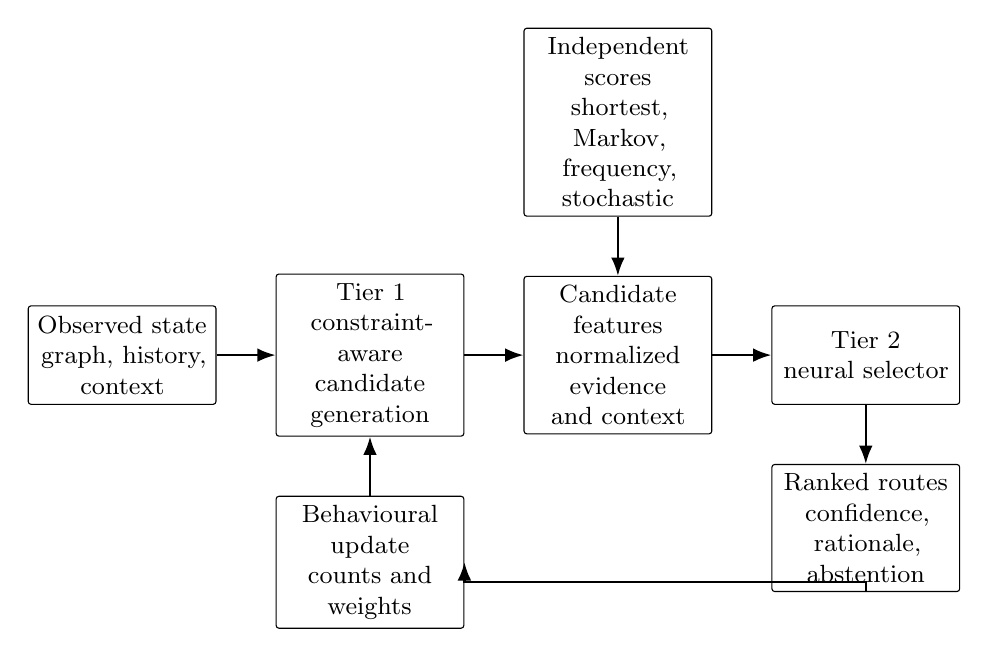
\begin{tikzpicture}[
  >=Latex,
  node distance=0.75cm and 0.75cm,
  box/.style={draw, rounded corners=1pt, align=center, minimum height=1.25cm, text width=2.15cm, font=\small},
  arrow/.style={->, thick}
]
\node[box] (observed) {Observed state\\graph, history,\\context};
\node[box, right=of observed] (tierone) {Tier 1\\constraint-aware\\candidate generation};
\node[box, right=of tierone] (features) {Candidate features\\normalized evidence\\and context};
\node[box, right=of features] (tiertwo) {Tier 2\\neural selector};
\node[box, above=of features] (scores) {Independent scores\\shortest, Markov,\\frequency, stochastic};
\node[box, below=of tiertwo] (ranked) {Ranked routes\\confidence, rationale,\\abstention};
\node[box, below=of tierone] (update) {Behavioural update\\counts and weights};

\draw[arrow] (observed) -- (tierone);
\draw[arrow] (tierone) -- (features);
\draw[arrow] (features) -- (tiertwo);
\draw[arrow] (scores) -- (features);
\draw[arrow] (tiertwo) -- (ranked);
\draw[arrow] (update) -- (tierone);
\draw[arrow] (ranked.south) |- ($(update.east)+(0,-0.25)$) -- (update.east);
\end{tikzpicture}
\caption{Conceptual separation of structural candidate generation from learned candidate selection. Feedback is defined only after a realized movement becomes observable.}
\label{fig:architecture}
\end{figure}

\subsection{Tier 1: Candidate Generation}

Tier~1 builds a compact but diverse set $\Ccal_t$. It starts with a minimum-resistance path and then generates loopless deviations using a $K$-shortest-path procedure in the style of Yen \cite{yen1971}. Independent components may contribute additional candidates:

\begin{itemize}
  \item the shortest physical or generalized-cost path;
  \item empirical Markov transitions and node-frequency proposals;
  \item Monte Carlo or stochastic-routing proposals;
  \item destination-progress and dynamic-edge proposals;
  \item graph-centrality or adaptive-transition proposals; and
  \item domain-specific constraints and node-elimination rules.
\end{itemize}

The tier deduplicates candidates, applies feasibility constraints, promotes diversity, and enforces the budget $K$. The selector can recover the realized route only if Tier~1 supplies an equivalent candidate. Candidate recall is therefore a separate object of evaluation.

\subsection{Historical Transition and Node-Frequency Priors}

For current node $u$ and possible successor $v\in N_t^+(u)$, let $n_0(u,v)$ be a population transition count and $n_a(u,v)$ an entity-specific count for entity $a$. With additive smoothing $\alpha>0$,
\begin{equation}
p_0(v\mid u)=\frac{n_0(u,v)+\alpha}{\sum_{j\in N_t^+(u)}n_0(u,j)+\alpha\lvert N_t^+(u)\rvert},
\end{equation}
\begin{equation}
p_a(v\mid u)=\frac{n_a(u,v)+\alpha}{\sum_{j\in N_t^+(u)}n_a(u,j)+\alpha\lvert N_t^+(u)\rvert}.
\end{equation}
Sparse entity histories should not override a more stable population model. Define a data-dependent confidence
\begin{equation}
c_a(u)=\frac{N_a(u)}{N_a(u)+\kappa},
\end{equation}
where $N_a(u)=\sum_jn_a(u,j)$ and $\kappa>0$ controls shrinkage. The blended pattern prior is
\begin{equation}
\widehat p_{\mathrm{hist}}(v\mid u,a)
=c_a(u)p_a(v\mid u)+\bigl(1-c_a(u)\bigr)p_0(v\mid u).
\end{equation}
This is the formal version of the design rule $\widehat P(\text{next}=v)=cP_{\mathrm{entity}}+(1-c)P_{\mathrm{base}}$. Node frequency provides a complementary prior:
\begin{equation}
f(v)=\frac{n(v)+\alpha_f}{\sum_{j\in V_t}n(j)+\alpha_f\lvert V_t\rvert}.
\end{equation}
Transition frequency answers where an entity goes after $u$, while node frequency describes which locations are visited often overall. Conflating them loses directional information.

\subsection{Contextual Next-Node Probability}

Let $D_t(v,g)$ be the remaining distance from $v$ to the target and define destination progress
\begin{equation}
\Delta_g(u,v)=D_t(u,g)-D_t(v,g).
\end{equation}
A local probabilistic movement rule is
\begin{align}
U_t(u,v)={}&-\beta\rho_t(u,v\mid z_t)
+\gamma\log\bigl(\widehat p_{\mathrm{hist}}(v\mid u,a)+\varepsilon\bigr)\notag\\
&+\delta\log\bigl(f(v)+\varepsilon\bigr)+\eta\Delta_g(u,v).
\end{align}
The resulting normalized probability is
\begin{equation}
P(v\mid u,z_t,a)=
\frac{\exp(U_t(u,v))}{\sum_{j\in N_t^+(u)}\exp(U_t(u,j))}.
\end{equation}
Equation~(17) imposes $\beta,\gamma,\delta,\eta\geq0$. Thus greater resistance lowers utility, while increases in historical familiarity, node frequency, and destination progress raise it, holding the other terms fixed.

\subsection{Independent Model Scores and Fixed Ensemble}

For candidate $r$, let $q_m(r,z_t)$ be the score returned by model $m\in\{1,\ldots,M\}$. After converting all scores so that larger is better and normalizing them within the candidate set, a fixed ensemble is
\begin{equation}
S_{\mathrm{fixed}}(r)=\sum_{m=1}^{M}\omega_m\widetilde q_m(r,z_t),
\qquad \omega_m\geq0, \qquad \sum_m\omega_m=1.
\end{equation}
The fixed score is transparent, but its weights do not change with context. A learned selector is introduced to model interactions among scores, state, and contextual features.

\subsection{Tier 2: Neural Candidate Selector}

The selector receives a candidate feature vector $\phi(r,z_t)\in\mathbb{R}^p$. Its components may include independent model scores, transition evidence, node frequency, graph structure, destination progress, time-dependent context, and the fixed ensemble. A one-hidden-layer realization is
\begin{equation}
h_r=\ReLU\bigl(W_1\phi(r,z_t)+b_1\bigr),
\end{equation}
\begin{equation}
\widehat y_r=\sigma\bigl(w_2^\top h_r+b_2\bigr),
\end{equation}
where $\widehat y_r$ estimates candidate correctness under a predeclared label definition. With binary label $y_r\in\{0,1\}$, the empirical cross-entropy objective is
\begin{equation}
\mathcal{L}=-\frac{1}{N}\sum_{i=1}^{N}
\left[y_i\log\widehat y_i+(1-y_i)\log(1-\widehat y_i)\right].
\end{equation}
The term two-tier refers to the full decision architecture---candidate generation followed by learned selection. Equation~(20) gives a compact selector realization; other differentiable ranking architectures may replace it without altering Tier~1.

Within one decision set, sigmoid outputs may be converted into a normalized candidate distribution using logits $\ell_r=\log(\widehat y_r/(1-\widehat y_r))$:
\begin{equation}
\pi(r\mid\Ccal_t,z_t)=
\frac{\exp(\ell_r/T)}{\sum_{r'\in\Ccal_t}\exp(\ell_{r'}/T)},
\end{equation}
where temperature $T>0$ is estimated on a calibration set. The predicted route is
\begin{equation}
\widehat r=\arg\max_{r\in\Ccal_t}\pi(r\mid\Ccal_t,z_t).
\end{equation}

\subsection{Confidence, Entropy, and Abstention}

Define confidence $c_t=\max_r\pi(r\mid\Ccal_t,z_t)$ and route entropy
\begin{equation}
H_t=-\sum_{r\in\Ccal_t}\pi(r\mid\Ccal_t,z_t)
\log\pi(r\mid\Ccal_t,z_t).
\end{equation}
The decision rule abstains or defers to a human analyst when
\begin{equation}
c_t<\tau_c \qquad \text{or} \qquad H_t>\tau_H,
\end{equation}
or when input freshness, graph coverage, or feature completeness falls below a declared threshold. This makes insufficient evidence an explicit model outcome.

\section{Algorithms}

\subsection{Prediction Procedure}

\begin{lstlisting}[style=pseudocode,caption={Abstract two-tier route-prediction procedure.}]
INPUT: dynamic graph G_t, start s, goal g, context z_t,
       entity a, candidate budget K, confidence threshold tau

1. Update edge feasibility and generalized resistance from z_t.
2. Remove nodes and edges that violate hard constraints.
3. Generate a minimum-resistance route from s to g.
4. Generate loopless K-path deviations; reject cycles and
   immediate backtracking.
5. Add valid candidates proposed by transition, node-frequency,
   stochastic, destination-progress, and adaptive-graph models.
6. Deduplicate candidates and retain a diverse budgeted set C_t.
7. For every route r in C_t:
     a. compute independent model scores;
     b. compute graph, history, state, and context features;
     c. compute fixed score S_fixed(r);
     d. compute neural score y_hat_r.
8. Normalize candidate scores to route probabilities pi(r).
9. If C_t is empty, inputs violate admissibility conditions,
   or max pi(r) < tau: ABSTAIN.
10. Otherwise return ranked top-K routes, confidence, uncertainty,
    and the feature-level rationale.
\end{lstlisting}

\subsection{Adaptive Update After Observation}

The mathematical update is defined only after the realized next node or route becomes observable.

\begin{lstlisting}[style=pseudocode,caption={Abstract behavioural and graph update.}]
INPUT: previous node u, realized next node v, entity a,
       context z_t, candidate predictions and labels

1. Increment population transition count n_0(u,v).
2. Increment entity transition count n_a(u,v).
3. Increment node visit count n(v).
4. Recompute smoothed transition and node-frequency priors.
5. Update time-dependent edge attributes and context freshness.
6. Add the completed decision and labels to the learning history.
7. On a controlled schedule, estimate or recalibrate parameters.
8. Compare a challenger rule with the current rule on a temporal
   holdout defined by the future evaluation protocol.
9. Adopt the challenger only if prespecified accuracy,
   calibration, coverage, and safety conditions are satisfied.
\end{lstlisting}

This delayed-update rule prevents future observations from entering the prediction that preceded them. It also separates the definition of online adaptation from any particular storage or software architecture.

\section{Terrain and Contour-Graph Extension}
\label{sec:terrain}

Terrain is relevant to surface routing, low-altitude operations, evacuation, search-and-rescue, and infrastructure restoration. Let a digital elevation model define elevation field $h(x,y)$. For an edge $e=(u,v)$ with horizontal distance $d(u,v)$, define signed grade
\begin{equation}
g_e=\frac{h(v)-h(u)}{d(u,v)+\varepsilon}
\end{equation}
and absolute slope $s_e=\lvert g_e\rvert$. Let $N_c(e)$ count contour-line crossings, $R_e$ measure local elevation roughness, and $X_e$ represent line-of-sight or exposure where appropriate. Normalize these quantities using parameters estimated on a training split or fixed physical-domain bounds declared before evaluation. A terrain term can be written
\begin{equation}
q_{\mathrm{terrain}}(e)
=a_s\widetilde s_e+a_c\widetilde N_c(e)
+a_r\widetilde R_e+a_x\widetilde X_e.
\end{equation}
In Equation~(28), the tilded variables are dimensionless normalized quantities, rather than raw slope, crossing counts, roughness, or exposure. With all four inputs oriented as resistance, $a_s,a_c,a_r,a_x\geq0$.

A contour-derived graph does not automatically treat contour lines as routes. Contours or raster elevation are transformed into traversable cells or segments; impassable gradients and barriers remove edges; normalized slope and crossing statistics become attributes; and the candidate generator operates on the feasible graph. Application-specific mobility knowledge is required to identify the coefficients. Equation~(28) is a designed module within the theoretical framework.

\section{Proposed Evaluation Framework}

This section defines methodology for a future empirical companion study. No quantity below is evaluated in the present paper.

\subsection{Candidate Coverage and Ranking}

Let $r_t^*$ be the realized route and $\Ccal_t$ the generated candidate set. Candidate recall is
\begin{equation}
\operatorname{Recall}_{\mathrm{cand}}
=\frac{1}{T}\sum_{t=1}^{T}\ind\{r_t^*\in\Ccal_t\}.
\end{equation}
Conditional top-$K$ selection accuracy is
\begin{equation}
\operatorname{TopK}
=\frac{\sum_t\ind\{r_t^*\in\operatorname{TopK}_t\}}
{\sum_t\ind\{r_t^*\in\Ccal_t\}}.
\end{equation}
Conditional selection accuracy can conceal poor candidate recall, so both quantities are required.

\subsection{Next-Node and Full-Route Accuracy}

For true next node $y_t$ and predicted next node $\widehat y_t$,
\begin{equation}
\operatorname{Accuracy}_{\mathrm{node}}
=\frac{1}{T}\sum_{t=1}^{T}\ind\{\widehat y_t=y_t\}.
\end{equation}
Exact-route accuracy is stricter:
\begin{equation}
\operatorname{Accuracy}_{\mathrm{route}}
=\frac{1}{T}\sum_{t=1}^{T}\ind\{\widehat r_t=r_t^*\}.
\end{equation}
When partial correctness has operational value, a study also reports prefix accuracy, normalized edit distance, edge overlap, and destination error. Manhattan distance may suit a grid; geographic settings typically require great-circle or network distance.

\subsection{Probabilistic Metrics}

For candidate distribution $\pi_t$, negative log-likelihood and multiclass Brier score are
\begin{equation}
\operatorname{NLL}=-\frac{1}{T}\sum_{t=1}^{T}\log\pi_t(r_t^*),
\end{equation}
\begin{equation}
\operatorname{Brier}=\frac{1}{T}\sum_{t=1}^{T}
\sum_{r\in\Ccal_t}\left(\pi_t(r)-\ind\{r=r_t^*\}\right)^2.
\end{equation}
For confidence bins $B_1,\ldots,B_B$, expected calibration error is
\begin{equation}
\operatorname{ECE}=\sum_{b=1}^{B}\frac{\lvert B_b\rvert}{T}
\left\lvert\operatorname{acc}(B_b)-\operatorname{conf}(B_b)\right\rvert.
\end{equation}
Calibration is assessed on data held out after model fitting. Temperature scaling provides a suitable baseline procedure \cite{guo2017}.

\subsection{Selective Prediction and Availability}

At confidence threshold $\tau$, define coverage
\begin{equation}
\operatorname{Coverage}(\tau)=\frac{1}{T}\sum_{t=1}^{T}\ind\{c_t\geq\tau\}.
\end{equation}
Selective risk is the error rate among non-abstained cases. A risk--coverage curve exposes that trade-off. Availability is reported separately as the fraction of decision times for which freshness, graph completeness, and feature validity permit any prediction.

\subsection{Standing Requirements for a Results-Bearing Companion Paper}
\label{sec:standing-requirements}

The framework becomes a results-bearing publication only after a companion study meets all of the following requirements:

\begin{enumerate}
  \item Run six methods---shortest path, most-frequent transition, population Markov, entity Markov, fixed ensemble, and neural selector---on one entity-grouped chronological split and identical candidate sets.
  \item Repeat neural training under at least ten prespecified seeds. Report the mean, standard deviation, and a confidence interval across those runs.
  \item Preserve decision-event identifiers. Candidate recall, next-node accuracy, and full-route accuracy receive separate definitions, denominators, and result tables.
  \item Estimate uncertainty over decision-event clusters. A future design containing only 87 candidate rows cannot treat those rows as independent observations or use them as the sole uncertainty basis.
  \item Conduct repeated live evaluations over a declared period. Report availability, failure rate, the freshness threshold and its units, and the distribution of time to staleness.
  \item Archive the exact split, prespecified seeds, prediction files, preprocessing queries, model artefacts, evaluation environment, package versions, and hardware specification.
  \item Resolve every experimental placeholder with a measured result before making an empirical claim. If the requirements remain incomplete, the submission stays explicitly within the framework/design category represented by this paper.
\end{enumerate}

The future study also includes feature ablations, measures candidate recall and latency as $K$ varies, and tests missing, delayed, contradictory, and stale inputs. All thresholds, exclusions, and success criteria are registered before model fitting.

\section{Applications and Boundaries}

The mathematical structure can support several domains, provided each receives its own graph, context variables, constraints, governance, and validation:

\begin{itemize}
  \item \textbf{Aviation:} forecasting likely next sectors, waypoints, diversions, or arrival paths for research and traffic analysis;
  \item \textbf{Search-and-rescue:} ranking probable movement corridors under terrain, weather, access, and last-known-position constraints;
  \item \textbf{Emergency evacuation and disaster logistics:} estimating feasible routes as roads, bridges, and supply conditions change;
  \item \textbf{Infrastructure restoration:} prioritizing access routes for repair teams and supplies;
  \item \textbf{Network and information systems:} predicting packet, service, or failure-propagation paths on logical graphs;
  \item \textbf{Commercial logistics:} predicting vehicle movement under time, cost, congestion, and service constraints; and
  \item \textbf{Defence decision support:} analysing possible aircraft, vehicle, troop, or logistical routes under authorized and lawfully obtained information.
\end{itemize}

Transfer across domains is architectural. It does not transfer empirical validity. Each application requires independently justified variables, resistance scales, data rights, adversarial tests, uncertainty thresholds, and human-oversight rules. High-consequence uses additionally require legal authority, provenance controls, a documented abstention policy, and a named decision owner.

\section{Limitations, Governance, and Future Work}

\subsection{Open Theoretical and Design Questions}

The framework leaves several issues open:

\begin{enumerate}
  \item \textbf{Known destination.} The target $g$ is supplied to the route model. Joint destination and route inference requires an additional latent-variable layer.
  \item \textbf{Candidate completeness.} Tier~2 cannot select a route absent from $\Ccal_t$. Formal guarantees relating candidate budget, diversity, and route recovery remain to be developed.
  \item \textbf{Identifiability.} Correlated resistance terms can admit multiple coefficient vectors with similar utilities. Normalization, regularization, and domain constraints are necessary, but a general identifiability result is unresolved.
  \item \textbf{Nonstationarity.} Transition patterns and edge conditions may drift. The update rule defines when feedback enters, while convergence and regret under changing graphs remain open.
  \item \textbf{Dependence and calibration.} Candidates within an event are coupled by construction. Calibration and uncertainty procedures must respect event-level dependence and distribution shift.
  \item \textbf{Computational scaling.} Candidate diversity improves coverage but increases search and scoring cost. Bounds linking $K$, latency, and recoverability require further analysis.
  \item \textbf{Semantic validity.} Risk, access, affiliation, safe-location, and exposure variables have no universal meaning. Their use depends on application-specific definitions and authoritative provenance.
\end{enumerate}

\subsection{Data and Model Governance}

Any future instantiation follows three policy principles. First, every decision is traceable to source records, feature times, candidate-generation rules, parameter versions, and the stated rationale. Second, entity histories receive access controls, retention limits, and purpose restrictions. Safety-sensitive attributes require an approved semantic definition and authoritative provenance. Third, disagreement among component models, missing context, and abstention remain visible to the human decision maker. Release, rollback, and override authority are assigned before deployment.

\subsection{Future Work}

The next theoretical steps are joint destination--route inference, guarantees for candidate coverage, identifiability analysis for generalized resistance, drift-aware updates, and computational bounds for the candidate budget. Robust extensions may also study adversarial observations, partially observed graphs, multiple interacting entities, and constrained multi-objective route distributions. Empirical work begins only under the standing design in Section~\ref{sec:standing-requirements}; those experiments belong in a separate companion paper.

\section{Conclusion}

This paper defines a route-prediction framework in which constrained graph search proposes feasible alternatives and a learned selector ranks them using historical, structural, geometric, and contextual evidence. Population and entity-specific histories are blended through shrinkage; resistance and context enter a sign-constrained utility; candidate scores form a normalized route distribution; and confidence, entropy, and abstention make uncertainty part of the decision rule.

The mathematical contribution includes the generalized resistance model, the two-tier probability construction, and the expected route-length bound between the shortest and longest candidates. The terrain module illustrates how a new resistance family can enter without changing the architecture. The evaluation section defines the evidence required to test the framework while keeping candidate coverage, selection quality, calibration, and availability distinct. As a framework/design paper, this manuscript makes no implementation or performance claim.

\appendix
\section{Notation Summary}

\begin{table}[htbp]
\centering
\begin{tabularx}{\textwidth}{>{\raggedright\arraybackslash}p{0.33\textwidth} X}
\toprule
\textbf{Symbol} & \textbf{Meaning} \\
\midrule
$G_t=(V_t,E_t,W_t)$ & Dynamic directed graph at time $t$ \\
$s,g$ & Known start and target nodes \\
$r=(v_0,\ldots,v_m)$ & Feasible route from $s$ to $g$ \\
$\Rcal_t(s,g)$ & Set of all feasible routes \\
$\Ccal_t$ & Finite candidate set supplied to the selector \\
$L_t(r)$ & Physical or network length of route $r$ \\
$\rho_t(e\mid z_t)$ & Context-dependent edge resistance \\
$C_t(r\mid z_t)$ & Generalized route cost \\
$p_0(v\mid u)$ & Population transition probability \\
$p_a(v\mid u)$ & Entity-specific transition probability \\
$c_a(u)$ & Confidence assigned to entity-specific history \\
$f(v)$ & Smoothed node-frequency prior \\
$q_m(r,z_t)$ & Candidate score from independent model $m$ \\
$S_{\mathrm{fixed}}(r)$ & Fixed weighted ensemble score \\
$\phi(r,z_t)$ & Neural selector feature vector \\
$\widehat y_r$ & Neural candidate-correctness score \\
$\pi(r\mid\Ccal_t,z_t)$ & Normalized route probability within the candidate set \\
$c_t,H_t$ & Maximum confidence and route entropy \\
\bottomrule
\end{tabularx}
\end{table}

\begin{thebibliography}{99}

\bibitem{dijkstra1959}
E. W. Dijkstra, ``A note on two problems in connexion with graphs,''
\emph{Numerische Mathematik}, vol.~1, pp.~269--271, 1959.
\href{https://doi.org/10.1007/BF01386390}{doi: 10.1007/BF01386390}.

\bibitem{yen1971}
J. Y. Yen, ``Finding the $K$ shortest loopless paths in a network,''
\emph{Management Science}, vol.~17, no.~11, pp.~712--716, 1971.
\href{https://doi.org/10.1287/mnsc.17.11.712}{doi: 10.1287/mnsc.17.11.712}.

\bibitem{guo2017}
C. Guo, G. Pleiss, Y. Sun, and K. Q. Weinberger,
``On calibration of modern neural networks,'' in \emph{Proceedings of the 34th International Conference on Machine Learning}, vol.~70, pp.~1321--1330, 2017.

\bibitem{yao2020}
R. Yao and S. Bekhor, ``Data-driven choice set generation and estimation of route choice models,''
\emph{Transportation Research Part C}, vol.~121, 102832, 2020.
\href{https://doi.org/10.1016/j.trc.2020.102832}{doi: 10.1016/j.trc.2020.102832}.

\bibitem{zhao2023}
Z. Zhao and Y. Liang, ``A deep inverse reinforcement learning approach to route choice modeling with context-dependent rewards,''
\emph{Transportation Research Part C}, vol.~149, 104079, 2023.
\href{https://doi.org/10.1016/j.trc.2023.104079}{doi: 10.1016/j.trc.2023.104079}.

\bibitem{qiu2024}
S. Qiu, G. Qin, M. Wong, and J. Sun,
``RoutesFormer: A sequence-based route choice Transformer for efficient path inference from sparse trajectories,''
\emph{Transportation Research Part C}, vol.~162, 104552, 2024.
\href{https://doi.org/10.1016/j.trc.2024.104552}{doi: 10.1016/j.trc.2024.104552}.

\bibitem{wang2024}
H. Wang, E. Moylan, and D. Levinson,
``Ensemble methods for route choice,''
\emph{Transportation Research Part C}, vol.~167, 104803, 2024.
\href{https://doi.org/10.1016/j.trc.2024.104803}{doi: 10.1016/j.trc.2024.104803}.

\bibitem{liang2020}
M. Liang, B. Yang, R. Hu, Y. Chen, R. Liao, S. Feng, and R. Urtasun,
``Learning lane graph representations for motion forecasting,'' in \emph{ECCV}, 2020.
\href{https://doi.org/10.1007/978-3-030-58536-5_32}{doi: 10.1007/978-3-030-58536-5\_32}.

\bibitem{salzmann2020}
T. Salzmann, B. Ivanovic, P. Chakravarty, and M. Pavone,
``Trajectron++: Dynamically-feasible trajectory forecasting with heterogeneous data,'' in \emph{ECCV}, 2020.
\href{https://doi.org/10.1007/978-3-030-58523-5_40}{doi: 10.1007/978-3-030-58523-5\_40}.

\bibitem{shi2022}
S. Shi, L. Jiang, D. Dai, and B. Schiele,
``Motion Transformer with global intention localization and local movement refinement,''
\emph{NeurIPS}, vol.~35, 2022.
\href{https://doi.org/10.52202/068431-0473}{doi: 10.52202/068431-0473}.

\bibitem{nayakanti2023}
N. Nayakanti, R. Al-Rfou, A. Zhou, K. Goel, K. S. Refaat, and B. Sapp,
``Wayformer: Motion forecasting via simple and efficient attention networks,'' in \emph{ICRA}, 2023.
\href{https://doi.org/10.1109/ICRA48891.2023.10160609}{doi: 10.1109/ICRA48891.2023.10160609}.

\bibitem{ettinger2021}
S. Ettinger et al., ``Large scale interactive motion forecasting for autonomous driving: The Waymo Open Motion Dataset,'' in \emph{ICCV}, 2021.

\bibitem{wilson2021}
B. Wilson et al., ``Argoverse 2: Next generation datasets for self-driving perception and forecasting,'' in \emph{Proceedings of the Neural Information Processing Systems Track on Datasets and Benchmarks}, vol.~1, 2021.

\bibitem{ngiam2022}
J. Ngiam et al., ``Scene Transformer: A unified architecture for predicting multiple agent trajectories,'' in \emph{ICLR}, 2022.

\end{thebibliography}

\end{document}
